Crear la siguiente configuración de red y utilizar RIP en las
máquinas uml

Comprobar las tablas de rutas y los mensajes intercambiados

  \begin{figure}[h]
    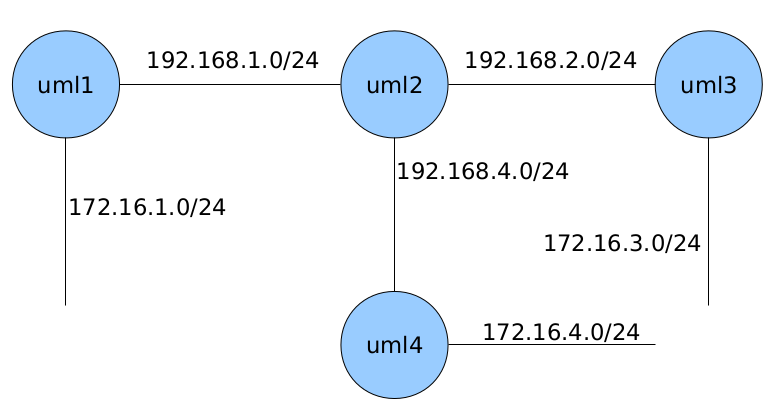
\includegraphics[width=10cm]{ripv1.png}
    \centering
  \end{figure}

  \begin{minted}{bash}
    # net.conf
    defsw br12 uml1.0 uml2.1
    defsw net1 uml1.1
    defsw br23 uml2.0 uml3.0
    defsw br24 uml2.2 uml4.0
    defsw net4 uml4.1
    defsw net3 uml3.1
  \end{minted}
  
  \begin{minted}{bash}
  # En cuanto se inician las UML, editar el fichero /etc/quagga/daemons la línea
  ripd=no
  # Por
  ripd=yes
  # A continuación restart del servicio
  systemctl restart quagga
  # Verificar que se ospfd está corriendo
  systemctl status quagga
\end{minted}
  
  \begin{minted}{lexer.py:IOSLexer -x}
    ! UML1 (zebra.conf)
    con[figure] t[erminal]
    int[erface] eth0
    ip addr[ess] 192.168.1.1/24
    no s[hutdown]
    q[uit]
    int[erface] eth1
    ip addr[ess] 172.16.1.1/24
    no s[hutdown]
    q[uit]
    ip f[orwarding]
    end
    w[rite]
  \end{minted}
  
  \begin{minted}{lexer.py:IOSLexer -x}
    ! UML1 (zebra.conf)
    con[figure] t[erminal]
    int[erface] eth0
    ip addr[ess] 192.168.1.1/24
    no s[hutdown]
    q[uit]
    int[erface] eth1
    ip addr[ess] 172.16.1.1/24
    no s[hutdown]
    q[uit]
    ip f[orwarding]
    end
    w[rite]
  \end{minted}
  
  \begin{minted}{lexer.py:IOSLexer -x}
    ! UML2 (zebra.conf)
    con[figure] t[erminal]
    int[erface] eth0
    ip addr[ess] 192.168.2.1/24
    no s[hutdown]
    q[uit]
    int[erface] eth1
    ip addr[ess] 192.168.1.2/24
    no s[hutdown]
    q[uit]
    int[erface] eth2
    ip addr[ess] 192.168.4.2/24
    no s[hutdown]
    q[uit]
    ip f[orwarding]
    end
    w[rite]
  \end{minted}
  
  \begin{minted}{lexer.py:IOSLexer -x}
    ! UML3 (zebra.conf)
    con[figure] t[erminal]
    int[erface] eth0
    ip addr[ess] 192.168.2.2/24
    no s[hutdown]
    q[uit]
    int[erface] eth1
    ip addr[ess] 172.16.3.1/24
    no s[hutdown]
    q[uit]
    ip f[orwarding]
    end
    w[rite]
  \end{minted}
  
  \begin{minted}{lexer.py:IOSLexer -x}
    ! UML4 (zebra.conf)
    con[figure] t[erminal]
    int[erface] eth0
    ip addr[ess] 192.168.4.1/24
    no s[hutdown]
    q[uit]
    int[erface] eth1
    ip addr[ess] 172.16.4.1/24
    no s[hutdown]
    q[uit]
    ip f[orwarding]
    end
    w[rite]
  \end{minted}
  
  \begin{minted}{lexer.py:IOSLexer -x}
    ! UML1 (ripd.conf)
    con[figure] t[erminal]
    router rip
      network eth0
      network eth1
      neighbor 192.168.1.2
      passive-interface eth0
      passive-interface eth1
      do w[rite]
  \end{minted}
  
  \begin{minted}{lexer.py:IOSLexer -x}
    ! UML2 (ripd.conf)
    con[figure] t[erminal]
    router rip
      network eth0
      network eth1
      network eth2
      neighbor 192.168.1.1
      neighbor 192.168.2.2
      neighbor 192.168.4.1
      passive-interface eth0
      passive-interface eth1
      passive-interface eth2
      do w[rite]
  \end{minted}
  
  \begin{minted}{lexer.py:IOSLexer -x}
    ! UML3 (ripd.conf)
    con[figure] t[erminal]
    router rip
      network eth0
      network eth1
      neighbor 192.168.2.1
      passive-interface eth0
      passive-interface eth1
      do w[rite]
  \end{minted}
  
  \begin{minted}{lexer.py:IOSLexer -x}
    ! UML4 (ripd.conf)
    con[figure] t[erminal]
    router rip
      network eth0
      network eth1
      neighbor 192.168.4.2
      passive-interface eth0
      passive-interface eth1
      do w[rite]
  \end{minted}
  
  Pruebas:
  \begin{minted}{lexer.py:IOSLexer -x}
    sh[ow] ip rip
    sh[ow] ip route
  \end{minted}